\chapter{How Power Systems Work and Why Balance Matters}
\chaptermark{How Power Systems Work}

Imagine your regional electric grid as a huge, humming engine. Complicated as it is, its fundamental job is balance: keeping exactly the right amount of power flowing at every moment. This chapter explains how power systems work, why that balance matters, and how Bitcoin mining can help maintain it.

\section{Electric Power System Basics}

Electric power systems have three main components: generation, \glossaryterm{transmission}{transmission}, and \glossaryterm{distribution}{distribution} (delivery to loads, the consumers of power). In simple terms, power plants generate electricity, step-up transformers raise it to high voltage, transmission lines carry it over long distances, and lower-voltage distribution networks finally deliver it to homes and businesses. Generation refers to producing electricity from energy sources (for example, burning natural gas or harnessing wind in a turbine). Transmission is the bulk transport of electricity at high voltages over regional distances (the tall tower lines you see crossing the countryside). High voltages are used because they allow efficient long-distance transfer with minimal losses. Distribution is the local delivery of power at lower voltages, after transformers step down the voltage, to neighborhoods, businesses, and individual consumers.
The largest consumers usually skip that last step. A mine of the size this book prices, like the 100~MW site of Chapter~\ref{ch:buying}, takes its power straight from the transmission system through its own substation. In the territory of Oncor, a Texas transmission and distribution utility, that means delivery above 60,000 volts \autocite{oncor2026retailtariff}. % src: oncor2026retailtariff sec. 6.2.2 Standard Voltages, p. 164 ("Transmission voltage is any one of the Company's standard voltages in excess of 60,000 volts"; standard transmission voltages 69, 138 and 345 kV) and sec. 6.1.1.1.7 Transmission Service, p. 80; "a substation of its own" is not the tariff's phrase but follows from its definitions on p. 164: primary voltage is delivery "after one Company transformation ... from a transmission voltage", while transmission-voltage delivery has no Company transformation, so the step-down transformer is the customer's; chapter 6 tab:btm-ledger (100 MW at transmission voltage in Oncor's territory)
Load (or demand) denotes the electricity being consumed by end-users: all the lights, appliances, machines, and devices drawing power at any given moment. All these pieces together form what's commonly called the grid, an interconnected network linking producers and consumers of electricity \autocite{EIAElectricDelivery}.

\begin{figure}[h]
    \centering
    \resizebox{\textwidth}{!}{% Original diagram (it replaced an unattributed PNG, since deleted).
% Generation -> transmission -> distribution -> load chain with
% step-up/step-down transformers drawn as overlapping circles, plus the
% transmission-level tap that serves large sites (mines, data centers,
% heavy industry) through their own step-down substation.
\begin{tikzpicture}[
  font=\small,
  stage/.style={draw=black!70, rounded corners=2pt, thick, align=center,
                minimum height=10mm, minimum width=23mm},
  xfmr/.style={circle, draw=black!70, thick, minimum size=4.2mm, inner sep=0pt},
  arr/.style={-{Stealth[length=2.2mm]}, thick, black!70},
  note/.style={font=\scriptsize, text=black!55, align=center}
]
  \node[stage] (gen)  at (0,0)    {Generation};
  \node[stage] (tx)   at (3.9,0)  {Transmission};
  \node[stage] (dist) at (7.8,0)  {Distribution};
  \node[stage] (load) at (11.7,0) {Load};
  \node[stage] (big)  at (3.9,2.5) {Large site};

  % step-up transformer between generation and transmission
  \node[xfmr] (t1a) at (1.75,0) {};
  \node[xfmr] (t1b) at (2.02,0) {};
  \draw[arr] (gen) -- (t1a);
  \draw[arr] (t1b) -- (tx);
  \node[note] at (1.885,-0.55) {step-up\\transformer};

  % step-down transformer between transmission and distribution
  \node[xfmr] (t2a) at (5.65,0) {};
  \node[xfmr] (t2b) at (5.92,0) {};
  \draw[arr] (tx) -- (t2a);
  \draw[arr] (t2b) -- (dist);
  \node[note] at (5.785,-0.55) {step-down\\transformer};

  \draw[arr] (dist) -- (load);

  % transmission-level tap: the large site's own step-down substation
  \node[xfmr] (t3a) at (3.9,1.115) {};
  \node[xfmr] (t3b) at (3.9,1.385) {};
  \draw[arr] (tx) -- (t3a);
  \draw[arr] (t3b) -- (big);
  \node[note, anchor=west] at (4.2,1.25) {site's own\\substation};

  % stage annotations
  \node[note] at (0,-1.25)    {power plants: gas, wind,\\solar, nuclear, hydro};
  \node[note] at (3.9,-1.25)  {high voltage\\(69--765 kV)};
  \node[note] at (7.8,-1.25)  {lower voltage\\(4--35 kV)};
  \node[note] at (11.7,-1.25) {homes, businesses,\\smaller industry};
  \node[note, anchor=west] at (5.2,2.5) {mines, data centers, heavy industry:\\served at transmission voltage};
\end{tikzpicture}
}
    \caption{Simplified diagram of an electric power system: generation, transmission, and distribution deliver electricity to loads. Large sites, mines among them, take their power straight from the transmission system through a substation of their own.}
    \label{fig:power_system}
\end{figure}

Because our society relies on electricity, power systems are designed with reliability in mind. Most local grids are tied together into larger networks so they can support each other. For example, utilities interconnect their systems so that if one area has a shortage or an outage, power can be rerouted from elsewhere to compensate. In North America, virtually all generators within a vast region operate synchronously as part of large interconnections (Eastern, Western, and Texas interconnections in the U.S.). This means the entire grid in each region runs at the same electrical frequency (60~Hz in the United States), and power can flow across state or regional lines as needed. These interconnections and built-in redundancies help ensure that failures (like a single power plant or line tripping offline) do not immediately lead to widespread outages. The grid is a single huge machine with many parts working together to keep your lights on.

\section{Balancing Supply and Demand in Real Time}

Electricity supply must always match demand in real time. Unlike some other commodities, electricity cannot be easily stored in large quantities (at least not yet on the scale of the whole grid), so generation and load must be balanced every second of every day. If consumers collectively need, say, 30,000 megawatts (MW) at a given moment, the connected power plants must produce roughly 30,000~MW in that moment. If generation and consumption fall out of balance, even for a short time, the stability of the grid is jeopardized. Grid operators (sometimes called balancing authorities) are responsible for monitoring this balance and adjusting generation output or shifting loads as needed to keep the two in sync.

The \glossaryterm{utility-frequency}{utility frequency} is a key indicator of that balance. In a synchronized AC grid, frequency is the number of alternating current cycles per second, measured in hertz (Hz). In the U.S., the standard frequency is 60~Hz, while in many other countries it is 50~Hz. When generation exceeds demand, the grid frequency will rise above its target (generators speed up); if demand exceeds generation, the frequency will drop below 60~Hz (generators slow down). The direction of frequency change reveals the imbalance. Frequency can settle below or above its target once supply and demand match again; returning it to the target takes a further control action. Operators use control systems and operating reserves to hold frequency very close to the 60~Hz setpoint at all times \autocite{NERCBalancingFrequency2021}.

\section{Slowing the Fall and Stopping It}
\label{sec:inertia}

When a big power plant trips offline, its output vanishes in an instant, but the frequency does not collapse in that instant.
The big synchronous generators on the grid (gas, coal, nuclear, hydroelectric) are several thousand tons of metal spinning in lockstep with all the others, often at 3,600 revolutions per minute, and that spinning mass stores energy \autocite{FERCNERCFeb2021,ercot2024asstudy}. % src: FERCNERCFeb2021 appendix E, appendix p. 19 (PDF p. 263): "synchronous generators are several thousand tons of mass in motion, often rotating at 3,600 revolutions per minute (at 60 Hz)"; ercot2024asstudy p. 25 (inertia "inherently provided by synchronous generators, such as gas, coal, nuclear, and hydro")
That stored energy is the grid's \glossaryterm{inertia}{inertia}: in the first seconds after a trip, the missing power is drawn out of the rotating machines themselves, they slow down, and the frequency falls with them \autocite{ercot2018inertia,NERCBalancingFrequency2021}. % src: ercot2018inertia p. 4 ("kinetic energy will automatically be extracted from the synchronous machines, causing them to slow down"); NERCBalancingFrequency2021 p. 7 (energy "flows from the rotating masses of the connected resources into the power system")
In the humming engine of this chapter's opening, inertia is the flywheel.
How fast frequency falls, the \glossaryterm{rate-of-change-of-frequency}{rate of change of frequency} (RoCoF), depends on how much power went missing and how much inertia is online to absorb the blow: the less inertia, the steeper the fall \autocite{ercot2018inertia}. % src: ercot2018inertia pp. 3-5 ("System inertia determines the initial rate of frequency decline after a sudden loss of generation"; "If system inertia is low, the RoCoF after an event is higher")
Solar panels, batteries and most wind turbines reach the grid through inverters, which keep whatever spins inside them out of step with the grid, and so add no inertia of their own. Only inverters built to be grid-forming, a newer design, answer a frequency drop at once, much as spinning mass does \autocite{nerc2021gfm}. % src: nerc2021gfm p. 13, Table 1.1 (grid-forming: "Inherently provides fast energy injection in the inertial timeframe"; grid-following: fast frequency response only "with a short time delay needed for frequency measurement and control response"); older fixed-speed wind turbines coupled directly to the grid do add some inertia (review comment 2026-10-10), hence "most"; rewritten 2026-10-12 after a review comment that inverter-based resources add no inertia anywhere unless grid-forming, not only on ERCOT's accounting
ERCOT counts all three as adding none, so its inertia rises and falls with the number and size of the spinning units online: typically 200 to 400 gigawatt-seconds (\mbox{GW-s}, the unit of that stored energy), lowest in spring and fall, when demand is low and wind and solar carry much of it \autocite{ercot2024asstudy}. % src: ercot2024asstudy pp. 25-26 (IBRs "namely wind, solar, and battery resources, do not provide inertia"; "typically between 200 GW-s and 400 GW-s depending on the number and size of synchronous generators that are online"; low inertia at low net load, "usually occur in the spring and fall"); attributed to ERCOT since 2026-10-10: older fixed-speed wind turbines coupled directly to the grid do add some inertia (review comment), while ERCOT's study counts wind among the inverter-based resources that provide none
ERCOT puts the safe floor at 100~\mbox{GW-s}; the lowest it had seen in the ten years to 2024 was 115~\mbox{GW-s}, in March 2022 \autocite{ercot2024asstudy}. % src: ercot2024asstudy pp. 25-26 ("critical inertia" of 100 GW-s, "the amount of inertia needed to maintain stability"; "lowest inertia that ERCOT has experienced in the last ten years has been 115 GW-s, which occurred in March 2022")

Inertia only slows the fall. Stopping it is the job of the first layer of frequency control, \glossaryterm{primary-frequency-response}{primary frequency response}: the governor on each generator, a speed regulator on its turbine, senses the falling frequency and opens the throttle in proportion to the error, with no instruction from anyone \autocite{NERCBalancingFrequency2021}. % src: NERCBalancingFrequency2021 pp. 8, 13-14 (PFR is "autonomous"; governors "supply more energy to the generators' prime movers"; droop sets the size of the response to the frequency error, typical slope 5 percent)
Conventional governors typically begin to respond about three and a half seconds after a trip, a new balance usually comes within twelve, and frequency then settles a little above its low point: primary response does not bring it back to 60~Hz \autocite{FERCNERCFeb2021,NERCBalancingFrequency2021}. % src: FERCNERCFeb2021 appendix E, appendix p. 19 ("conventional generators typically begin their governor response in about 3.5 seconds"; new balance "usually in less than 12 seconds"), appendix p. 18 (Value B, the post-disturbance stabilized frequency); NERCBalancingFrequency2021 p. 8 ("primary control will not return frequency to nominal, but only arrest and stabilize it"), p. 13 (Point C the nadir, Value B the settling frequency) and p. 17 (governors in the East do not provide the "Point C to B" recovery of frequency as they do in the other interconnections, ERCOT among them)
Low inertia squeezes that window hard. The \glossaryterm{ferc}{Federal Energy Regulatory Commission (FERC)} regulates interstate electricity transmission and wholesale sales; the \glossaryterm{nerc}{North American Electric Reliability Corporation (NERC)} develops and enforces bulk power system reliability standards \autocite{fercrole2026,nercrole2026}. Their staff report on Winter Storm Uri studied a 2,750~MW loss met by conventional governors alone, with no fast frequency response, and asked how much primary response would hold frequency to roughly the same low point at different loads. % src: FERCNERCFeb2021 appendix E, appendix p. 21 (PDF p. 265): three load/inertia cases, a 2,750 MW resource loss in each, PFR adjusted to hold the nadir at approximately the same frequency, "the PFR is from conventional generation without any fast frequency response"
At the highest load and inertia it modeled, the answer was 1,300~MW; at a load of 17~GW it was 4,700~MW, because the fall bottomed out after about 3.6 seconds, just as those governors begin to move \autocite{FERCNERCFeb2021}. % src: FERCNERCFeb2021 appendix E, appendix p. 21 (PDF p. 265): case 1 highest load and inertia, nadir about 10 s, 1,300 MW of PFR; case 3 load 17 GW, nadir about 3.6 s, 4,700 MW of PFR; appendix p. 19 (governors begin in about 3.5 s)
That is why the Responsive Reserve of Chapter~\ref{ch:ancillary}, ERCOT's fastest reserve, takes batteries and loads that trip on a relay (they act within half a second) alongside the governors, and why ERCOT buys more of it in the hours when history says inertia runs low \autocite{ercot2024asstudy}. % src: ercot2024asstudy p. 2 (RRS quantity varied "by hour, based on the historic inertia in that hour") and p. 7 ("RRS quantities are set based on historic inertia"; RRS-UFR from Load Resources below 59.7 Hz); chapter 7 RRS sub-forms (FFR 0.25 s, UFR 0.5 s)

The second layer returns frequency to its target. ERCOT's \glossaryterm{load-frequency-control}{Load Frequency Control}, its name for automatic generation control (AGC), runs from the control room and over the following minutes moves the generators and controllable loads paid to follow its signal (the Regulation reserve of Chapter~\ref{ch:ancillary}) until frequency is back at 60~Hz \autocite{NERCBalancingFrequency2021,FERCNERCFeb2021,potomac2026somercot}. % src: NERCBalancingFrequency2021 pp. 8-10 (secondary control in the "minutes" time frame, mostly through AGC; it "returns the frequency to nominal once primary control has arrested and stabilized it"; Table 1.1, secondary 1-10 minutes); FERCNERCFeb2021 appendix E, appendix p. 17 (PDF p. 261: in ERCOT frequency is "maintained through the automatic generation control (AGC) system"); potomac2026somercot p. 38 (Regulation "responds to Load Frequency Control (LFC), which sends instructions every four seconds to increase or decrease generation or demand"); chapter 7 Regulation
The third layer, from about ten minutes to hours, replaces what was lost: it starts and redispatches plants and calls on demand response so that the fast reserves are free for the next trip. Its tools include the \glossaryterm{ercot-contingency-reserve-service}{ERCOT Contingency Reserve Service (ECRS)}, a reserve deployable within ten minutes, and the Non-Spin reserves of Chapter~\ref{ch:ancillary}. When nothing else is left, operators order load shedding to win reserves back \autocite{FERCNERCFeb2021,NERCBalancingFrequency2021}. % src: FERCNERCFeb2021 appendix E, appendix p. 17 (tertiary control "redispatches generation, starts more generation, or calls on demand response to restore frequency responsive reserves"; "may include manual shedding of load"); NERCBalancingFrequency2021 p. 10 (Table 1.1, tertiary "10 Minutes-Hours"); chapter 7 ECRS (ten minutes, called to restore the crash barrier after it has been used) and Non-Spin (thirty minutes)
Beneath all three sits an automatic last resort, \glossaryterm{under-frequency-load-shedding}{under-frequency load shedding}: relays on local utilities' circuits that disconnect blocks of customers by themselves, at least five percent of load when frequency reaches 59.3~Hz and more in steps below that \autocite{FERCNERCFeb2021}. % src: FERCNERCFeb2021 p. 44 (ERCOT UFLS: at least 5 percent of load at 59.3 Hz, 15 percent at 58.9 Hz, 25 percent at 58.5 Hz)

Uri, the first case study below, was not a failure of inertia: during the frequency emergency in the small hours of February 15, ERCOT's inertia stayed between 254 and 349~\mbox{GW-s}, far above the floor \autocite{FERCNERCFeb2021}. % src: FERCNERCFeb2021 p. 138 (1-second inertia data "ranged from 254 GW-seconds to 349 GW-seconds, well above ERCOT's critical inertia level")
What ran short was the reserve that stops the fall \autocite{FERCNERCFeb2021}. % src: FERCNERCFeb2021 p. 137 (Physical Responsive Capability 1,044 MW at the 1:54 a.m. low point, against the 2,300 MW minimum responsive reserve requirement of p. 134) and p. 138 (responsive reserves below 1,430 MW for about 4.5 hours on February 15; "What-if" box: had a large unit tripped while Physical Responsive Capability was low, reserves "may have been insufficient to arrest the frequency decline above the first stage of underfrequency load shedding")

\section{When the Grid Loses Balance: Blackout Case Studies}

The grid cannot leave a power mismatch unaccounted for. Supply must cover consumption and losses; storage helps only by absorbing or supplying the difference. In the first moments of an imbalance, the rotating machines also act as an energy store: a shortfall draws down their kinetic energy and slows them, while a surplus adds energy and speeds them up. Frequency is the visible indicator of that changing speed, rather than the original cause of the mismatch \autocite{NERCBalancingFrequency2021}.

But frequency is also a physical operating condition. Prolonged low frequency can expose turbine blades to damaging vibration and fatigue, and reduced-frequency operation can cause thermal damage. Excessively high frequency means excessive rotational speed, which can also damage the machinery. Small, brief departures are expected; severity and duration determine the danger. Protective relays disconnect a unit before its operating limits are exceeded, but losing generation during a shortage deepens that shortage and can set off further trips. Restoring balance protects both the machines and the customers they supply \autocite{nerc2015protection,nerc2025largeloads}.

Even in well-managed power systems, extreme or unexpected events can force supply and demand out of balance, leading to outages. The two cases below are the Texas blackouts of 2021 and the 2003 blackout across the northeastern United States and Ontario.

\subsection{ERCOT (Texas) 2021 Winter Storm Blackouts}

In February 2021, Texas experienced an unprecedented winter storm (Winter Storm Uri) that led to one of the worst grid crises in U.S. history. Temperatures plunged far below normal, causing heating demand to skyrocket and simultaneously knocking out a huge portion of power generation capacity (as natural gas wells froze, plant equipment failed, wind turbines iced over, etc.). The result was a massive imbalance: at the event's worst, about 52~GW, nearly half of ERCOT's installed generation capacity, was forced offline \autocite{ERCOTUpdate2021}. % src: ERCOT Apr 27, 2021 update: max 52,037 MW unavailable (Feb 16, ~8:00 a.m.); ERCOT's initial Feb 24 figure was 52,277 MW = 48.6% of 107,514 MW installed
Nor could Texas borrow its way out: ERCOT's ties to other grids can import at most about 1,220~MW, while the grid operators next door in the Eastern Interconnection, facing the same storm, were importing nearly 13,000~MW from farther east at the peak \autocite{FERCNERCFeb2021}; Chapter~\ref{ch:ercot} explains why the Texas grid stands so nearly alone. % src: FERCNERCFeb2021 p. 14 (ERCOT "can only import slightly more than 1,000 MW over its direct current ties"; east-to-west transfers into MISO "peaked at nearly 13,000 MW on February 15") and p. 127 fn. 197 ("maximum total import limitation of only 1,220 MW"; MISO and SPP "collectively imported nearly 13,000 MW"; more ERCOT imports "likely would have decreased" what MISO and SPP could import); chapter 3 island grid (ercot2025gridinsightsdcties, 1,220 MW over three DC ties and one variable-frequency transformer, hence "ties" rather than FERC's "direct current ties")
In the early morning of February 15, with generators tripping in rapid succession, system frequency fell through the critical 59.4~Hz mark at 1:51~a.m.\ and bottomed at 59.304~Hz three minutes later \autocite{FERCNERCFeb2021}. % src: FERC/NERC staff report p. 137; ERCOT's own board deck says 59.302 Hz; 2 mHz apart, we use the FERC/NERC figure
That low point sat four thousandths of a hertz above the first step of under-frequency load shedding, close enough that relays cut off about 276~MW of customers by themselves \autocite{FERCNERCFeb2021}. % src: FERCNERCFeb2021 p. 137 ("Approximately 276 MW of load tripped by UFLS relays at this time, although system frequency was not actually recorded as at or below 59.3 Hz"); 59.304 minus 59.300 is 0.004 Hz
The 59.4~Hz mark matters because of protective relays: if frequency stays at or below 59.4~Hz for more than nine minutes, generators are allowed to trip themselves offline automatically. That, after another four and a half minutes below the line, would have removed roughly another 17~GW of generation and risked a blackout of the whole ERCOT grid \autocite{FERCNERCFeb2021}. % src: PRC-024-2 Attachment 1, ERCOT Interconnection (<=59.4 Hz, 540 s) and FERC/NERC p. 44; p. 137 ("approximately 17,000 MW ... could potentially cause a complete blackout of the ERCOT Interconnection"); p. 239 ("if ERCOT had remained below 59.4 Hz for an additional four and a half minutes it would have lost approximately 17,000 MW ... and risked a potential blackout"); p. 230. The report never says almost certain: its modality is "potentially" and "risked a potential", and the stronger form was cut on 2026-09-20
Operators fought the drop with emergency load shedding (rolling blackouts): 1,000~MW ordered when the emergency was declared at 1:20~a.m., 5,000~MW by 1:50, 8,500~MW by 1:55, and a maximum of 20,000~MW later that day \autocite{FERCNERCFeb2021,ArgonneERCOT2021}. % src: FERC/NERC pp. 135-138 load-shed sequence (EEA3 declared 1:20 a.m.)
It worked: frequency climbed back above 59.4~Hz at 1:55~a.m., after four minutes and 23 seconds below the line, roughly half the time the relays would have waited \autocite{FERCNERCFeb2021}. % src: "remaining below 59.400 Hz for four minutes and 23 seconds" (p. 137). The often-quoted "4 minutes and 37 seconds" was stated orally by ERCOT's CEO (Feb 24-25, 2021) but contradicts both written primary sources; do not use it
ERCOT's chief executive later said the grid had been ``seconds and minutes'' from a catastrophic failure that could have left most of Texas dark for weeks \autocite{Douglas2021Seconds,MagnessTestimony2021}. % src: Texas Tribune, Feb 18, 2021; Magness written House testimony, Mar 24, 2021 ("power could have been out for 90% of Texans for weeks")
By deliberately cutting power to millions of customers, operators saved the rest of the system from an uncontrolled cascade.

\begin{figure}[h]
    \centering
    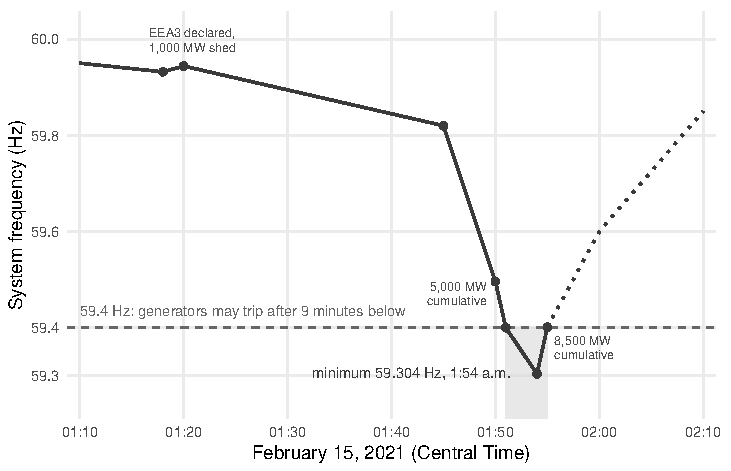
\includegraphics[width=\textwidth]{images/uri_frequency}
    \caption{ERCOT system frequency during the critical hour of February 15, 2021. Schematic: the line interpolates between values reported in the FERC/NERC staff report \autocite{FERCNERCFeb2021}; the recovery path after 1:55~a.m.\ is indicative. The frequency spent 4~minutes 23~seconds below the 59.4~Hz relay threshold.} % fig-src: analysis/figures/fig_ch2_uri_frequency.R
    \label{fig:frequency_drop}
\end{figure}

The human and economic impact was enormous. At the peak of the crisis about 4.5 million Texas homes and businesses were without power \autocite{CascadingRisks2021}, many for several days in freezing conditions. Tragically, the outage contributed to hundreds of deaths \autocite{DSHSWinterStormMortality2021}. The grid itself survived, thanks to those controlled outages. Over the following days (February 15--18), ERCOT worked to bring generation back and incrementally restore power. But until supply could meet demand again, utilities had to rotate outages to keep the reduced supply and high demand in balance.

\subsection{The 2003 Northeast Blackout}

On August 14, 2003, a sunny afternoon, a combination of technical glitches and human errors led to a cascading blackout across much of the Northeastern United States and Ontario, Canada. The trouble began when a series of FirstEnergy's high-voltage lines in northern Ohio tripped after contacting overgrown trees in their rights-of-way; the first was carrying well under half of its rated load, so this was a maintenance failure, not an overload \autocite{OutageTaskForce2004}. % src: Task Force Final Report pp. 17-19, 57-58: three 345-kV lines + one 138-kV faulted on tree contact; Harding-Chamberlin at 44% of rating; "overgrown trees, as opposed to excessive conductor sag"
Alone, those line losses would have been manageable. But FirstEnergy's control-room alarm system had silently failed almost an hour before the first line went down, so its operators did not know anything was wrong \autocite{OutageTaskForce2004}. % src: alarm and logging software failed 14:14 EDT; first tree contact 15:05 EDT; operators and IT support both unaware (pp. 51-53)
Power that had flowed on the failed lines shifted onto neighboring lines, which in turn overloaded and tripped in a chain reaction. Within minutes, a cascading failure was underway: as major transmission corridors went down, generators and loads across the region fell out of sync.

The disturbance rippled across the Northeast and parts of the Midwest and Canada, blacking out an estimated 50 million people and 61{,}800~MW of load in eight U.S. states and Ontario \autocite{OutageTaskForce2004}. % src: Task Force Final Report p. 1
In metropolitan areas like New York City, Cleveland, Detroit, and Toronto, power went out in a cascade that afternoon; parts of the United States waited four days for power, and parts of Ontario endured rolling blackouts for more than a week \autocite{OutageTaskForce2004}. The frequency in the affected areas plummeted as large power plants automatically shut down to protect themselves; in response, system protections began severing parts of the grid from each other to contain the collapse. The 2003 Northeast Blackout illustrated how interconnections meant to provide support can, under rare failure conditions, transmit disturbances far and wide. Its most lasting legacy was regulatory: the blackout led directly to mandatory, federally enforceable reliability standards for the North American bulk power system \autocite{OutageTaskForce2004,EPAct2005}. % src: Task Force Recommendation 1 (p. 140); EPAct 2005 sec. 1211 created FPA sec. 215; NERC certified as ERO 2006, standards mandatory June 2007

In Texas in 2021, supply crashed below demand; in the Northeast in 2003, uncontrolled power flows and losses caused parts of the Eastern Interconnection to fall out of sync. In each case, the grid's last-resort safety nets (automatic relays and operator-ordered outages) kicked in to try to stop the problem, but not before many customers were left in the dark.

\subsection{Why Recovery Takes Days or Weeks}

Once a grid has collapsed, why does it take days or even weeks to turn everything back on?

The core problem is that a power plant needs electricity before it can produce electricity. Fuel pumps, control systems, cooling equipment: all of it runs on station power that normally comes from the grid itself. When the grid is dead, most plants cannot start at all. Restoring a collapsed system therefore begins with a handful of designated \glossaryterm{black-start}{black start} units, typically hydroelectric plants or gas turbines with their own on-site generators, that can start with no outside power \autocite{NERCEOP005}. % src: NERC EOP-005-3, System Restoration from Blackstart Resources
Operators use them to energize pre-planned ``cranking paths'': transmission corridors that carry station power to larger plants, which then start up, pick up a small block of customers, and extend the electrified island outward \autocite{NERCEOP005}.

The balance rule from earlier in this chapter applies at every step. Each block of reconnected customers must be matched by generation already running, and a reconnected block briefly draws more than its normal share, because every thermostat and compressor in a cold, dark city switches on at once (operators call this cold-load pickup). Reconnect too much at once and the frequency of the young island collapses again, undoing hours of work. Separate islands must also be matched in frequency and voltage before they can be joined. Rebuilding a large grid is a sequence of thousands of careful, largely manual steps, which is why ERCOT's leadership estimated that a full black start of the Texas grid in 2021 would have left most of the state dark for weeks \autocite{MagnessTestimony2021,Douglas2021Seconds}. % src: Magness written House testimony (power out for 90% of Texans for weeks); Texas Tribune, Feb 18, 2021


\section{How Bitcoin Mining Can Support Grid Stability}

For the grid, Bitcoin mining is a highly \glossaryterm{flexible-load}{flexible} and controllable load: miners can rapidly scale down or shut off their power usage when needed. This flexibility means that, under the right incentives, Bitcoin miners can act as a kind of \glossaryterm{demand-side-reserve}{demand-side reserve} for the grid, helping balance supply and demand and prevent blackouts.

During normal times, miners operate around the clock, using electricity (often wherever it's cheapest or most abundant). But during grid stress events, say a hot summer afternoon when air conditioning load is at its peak or an unexpected power plant outage, miners can stop within minutes, freeing up electricity capacity to serve other critical needs. The industry calls this \glossaryterm{curtailment}{curtailment}, whoever sets it off: the site reading a price, or ERCOT or a generator sending an instruction the site has agreed to follow. Where it matters which of those happened, this book says \glossaryterm{pause}{pause} for the machine's own act. Nothing flows back into the grid when a mine stops; the generation it was using is simply free for everyone else, which has the same balancing effect as adding supply. A concrete example occurred in Texas in July 2022. Faced with record-breaking heat and electricity demand, over 95~percent of industrial-scale Bitcoin mines in Texas voluntarily paused during peak hours, freeing more than 1,000~MW of generation for other customers, according to the Texas Blockchain Council \autocite{TexasTribuneCrypto2022}. % src: TBC president Lee Bratcher, quoted in Chiu (Washington Post via Texas Tribune, Jul 15, 2022); industry self-report, not ERCOT-verified; Bratcher's own words were "push over 1,000 [megawatts] back into the grid", not repeated in prose because a load that stops injects nothing (glossary, load)
The council estimated that Texas miners curtailed more than 50,000~MWh over the month \autocite{UtilityDiveBitcoin2022}. % src: TBC statement reported by Utility Dive, Oct 19, 2022
That 1,000~MW was about 1.3~percent of ERCOT's heaviest demand hour that summer, enough to help the grid through the tightest hours without more severe emergency measures. The heaviest hour came on July 20, 2022, when demand across the grid averaged about 79,800~MW \autocite{EIAErcotPeak2023}. % src: EIA Today in Energy, Jul 26, 2023 (todayinenergy id=57240): "Previously, ERCOT's record for hourly demand was 79,830 megawatthours (MWh) on July 20, 2022." Chart note on the same page: hourly values "may differ from an instantaneous peak in demand", so MWh delivered in one clock hour = average MW sustained across that hour, which is why the prose says averaged and not peaked; 1,000/79,830 = 1.25%. Window is deliberately "that summer", not "on record": id=57240 shows 79,830 broken repeatedly in Jun-Jul 2023 (82,579 MWh on Jul 18, 2023), and EIA id=67906 (Jul 2026) gives 85.5 GW on Aug 10, 2023 and 91.1 GW on Jul 22, 2026

Winter tells the same story. In January 2024, Winter Storm Heather pushed ERCOT to five all-time winter demand records in four days, peaking at 78,349~MW on the morning of January 16 \autocite{ERCOTPeakRecords2024}, while the cold forced roughly 3,000~MW of additional generation outages \autocite{ERCOTMonthlyJan2024}. % src: 78,349 MW is the settled figure on ERCOT's 2024 Peak Demand Records page, unasterisked (ERCOT asterisks records pending settlement); the Jan-2024 Monthly prints 78,138 MW and labels its recap preliminary, so it carries the outages only; prior record 74,525 MW (Elliott, Dec 2022); Heather's record was itself surpassed by Winter Storm Kingston, Feb 20, 2025 (80,560 MW official)
ERCOT issued two conservation appeals and credited demand reductions, including by large flexible customers, with helping it avoid emergency operations \autocite{ERCOTConservation2024}. Bitcoin miners were a visible part of that response: network hashrate fell by roughly a quarter as Texas fleets paused \autocite{Hunt2024Hashrate}, and Riot Platforms alone earned \$3.3~million in curtailment and demand-response credits that month \autocite{Riot2024Jan}.
By the Texas Blockchain Council's own reckoning, wholesale prices during Heather's worst three days averaged only about \$100 per megawatt-hour, so much of Heather's curtailment was a response to prices, as Part~III examines in detail \autocite{Bratcher2024Data}. % src: Bratcher2024Data (TBC blog, Lee Bratcher, Jan 26 2024; verified at origin 2026-09-14): "The average settlement price of power on the wholesale market in ERCOT during the worst three days of the storm was $100.76 per MWh"; industry advocacy, affiliation now named in prose per source rule 4. TBC does not say which three days, so the window stays unnamed here per rule 5. Cross-check kept out of prose because the window is ours, not the monitor's: potomac2024som Table 8, p. 73 gives daily average RT prices across ERCOT's official Heather window of Jan 13-17 ($3.66, $70.78, $88.02, $148.71, $27.49); the mean of Jan 14-16 is $102.50 but Jan 15-17 is $88.07, so the agreement is window-dependent and the SOM never mentions Heather. Do NOT print TBC's companion claim that prices "never went over $600 per MWh": ERCOT Monthly Jan 2024 p. 4 shows a day-ahead price of about $1,900/MWh at the Jan 16 morning interval and System Lambda of about $1,134/MWh at the Jan 16 evening interval
Miners curtailed again during two winter storms in January 2025, mostly on price: Riot booked \$3.6~million in company-wide power credits for the month, of which \$3.2~million was curtailment and \$0.4~million came from formal ERCOT and MISO demand response programs, against \$1.0~million in December \autocite{Riot2025Jan}. The release does not split those demand-response credits between the markets. ERCOT called for no conservation during either storm and reported adequate supply to meet all demand \autocite{ERCOTMonthlyJan2025}. The flexibility works when the grid is merely strained, not only when it is breaking. % src: Riot Jan-2025 release (Feb 4, 2025) table: Power Credits $3.2M (fn 5, "Estimated power curtailment credits") vs $0.8M Dec-2024; Demand Response Credits $0.4M (fn 6, ERCOT and MISO programs); Total Power Credits $3.6M vs $1.0M Dec-2024 and $3.3M Jan-2024, so the $3.6M here is the same series as the $3.3M cited above for Jan 2024. ERCOT Monthly Jan 2025 (Feb 6, 2025) p.3 "January Winter Storms Recap": "The grid operated reliably during both winter storms with adequate supply to meet all demand"; "there was not a need to call for conservation and no outages were due to grid-wide reliability issues". Storms Cora (instantaneous peak 68,615 MW) and Enzo (77,758 MW). Do NOT restore "no grid emergency at all": same page records a transmission emergency in South and Southeast Texas, 5 a.m. to 1 p.m. Jan 21, about 29 iced lines, no controlled outages. The old comment's quote "less severe than recent historical winter storms" is not in that report and was dropped. Luxor cite removed earlier; Luxor banned as a source by the author, 2026-08-22

In January 2026, Winter Storm Fern brought another large response from flexible loads. The storm froze two-thirds of the country, and ERCOT's post-storm analysis estimated that underlying demand on the worst morning reached 84,558~MW, far past the all-time winter record and about 9,000~MW above what the meters actually recorded; the grid came through with no emergency alert, no conservation appeal, and no load shed \autocite{ERCOTMonthlyJan2026}. % src: ERCOT Monthly Jan 2026 (Feb 13, 2026), read at origin September 15, 2026: "the adjusted Monday morning peak was estimated at 84,558 MW" when the listed reductions are added back; those reductions sum to about 8,965 MW, hence "about 9,000 MW". The report gives NO metered peak; an earlier draft printed 75,572 MW, which appears in no ERCOT document and does not reconcile with the report's own arithmetic. Standing winter record 80,560 MW (Winter Storm Kingston, Feb 20, 2025, ERCOT records page); DOE issued a precautionary FPA 202(c) order Jan 24-27 that ERCOT never needed to invoke
The difference was flexible load stepping aside, and ERCOT itself did the accounting: roughly 4,100~MW of the reduction came from cryptocurrency miners, second only to the oil and gas sector and ahead of every other industry ERCOT counted, and more than twenty times what conventional data centers contributed \autocite{ERCOTMonthlyJan2026}. % src: same report: ~4,200 MW oil & gas, ~4,100 MW crypto, 420 MW steel, 170 MW data centers, 75 MW hydrogen/electrofuels; 4,100/170 = 24x
The response was visible in the Bitcoin network itself: roughly 200~EH/s went offline at U.S.-facing mining pools, average block times stretched to about 12.4 minutes against the protocol's 10-minute target, and the next difficulty adjustment was the largest downward move since China's 2021 mining ban. The adjustment after it more than made up the loss, up 14.7~percent, to about 2~percent above its level before the storm, as the machines returned \autocite{TheBlockFern2026,TheBlockDifficulty2026,BraiinsInsights}. % src: 200 EH/s offline and average block times "climbing to roughly 12.4 minutes" (The Block, Jan 26, 2026; theblock.co 403s to automated clients, read at the Wayback capture of 2026-02-09, retrieved 2026-09-14). 12.4 min implies hashrate about 19% below the difficulty-implied level (10/12.4 = 0.81); the Braiins Insights 1y series (7-day means) agrees in direction, and a sustained 40% drop would instead give about 16.7-minute blocks. -11.16% Feb 7 (The Block; Braiins Insights: 141.67 -> 125.86 T); rebound +14.73% to 144.40 T ~Feb 19-21 (Braiins Insights 1y series, verified 2026-08-22). NOT a record: ATH was 149.30 T in early Dec 2025; the old "snapping back to a record" claim was Luxor-sourced and wrong; Luxor banned as a source (author, 2026-08-22). CUT 2026-09-14: the "40% / ~455 EH/s trough" was a day-scale CoinWarz estimate reaching the book via CryptoSlate (Radmilac2026Fern), implying a ~1,138 EH/s baseline no series the book uses reproduces, in an article whose pool chart is sourced to banned Hashrate Index; cut under book-sources rule 6, cite dropped, entry removed from references.bib. Do NOT print a Braiins Insights percentage for this dip: three separate pulls on 2026-09-14 returned Jan 31 = 866.4 / 876.0 / 877.9 EH/s, giving -16.8% / -16.4% / -15.8% from Jan 24, so the figure is not reproducible at the precision print requires; 141.67 -> 125.86 -> 144.40 T, 144.40 / 141.67 = 1.0193, so about 2 percent above the pre-storm level; until 2026-10-10 "clawed back most of the lost ground" (review comment)
ERCOT's board chairman publicly credited the voluntary reductions by miners and data centers \autocite{FermanMalik2026}.

Bitcoin mining is suited to this role because it is an interruptible load by design. Stopping mining operations for a few hours doesn't ruin any product or inconvenience residential customers; it simply delays hashing, which miners accept when they are compensated for it, or when power prices are high. Miners describe their flexible load as a ``demand-side battery'': it soaks up excess power when supply is abundant (for instance, at night when wind farms might otherwise be curtailed) and shuts off on short notice when the grid is strained. The analogy has a limit: a battery can send back what it stored, while a mine stores nothing and can only stop drawing. Large mining farms can participate in demand response programs, getting paid to reduce consumption during grid emergencies just as industrial factories have long done. ERCOT has confirmed that miners ``respond during grid events by rapidly reducing their electric use,'' including during Uri \autocite{UtilityDiveBitcoin2022}.

Bitcoin mining can help address grid challenges alongside energy storage, other flexible industrial loads, and fast-ramping generation. A grid operator can achieve the same balancing effect as adding supply by curtailing a batch of miners that has signed up for it. As grids add more variable renewable generation and reserve margins tighten, a large consumer that can vanish in minutes becomes increasingly valuable. How miners are actually paid for that flexibility, through energy prices, ancillary services, and demand response programs, is the subject of Part~III.
